\section{Assignment 6}

\subsection{Implement the Scattering-based bilateral teleoperation architecture for the F-P and P-P cases}

\begin{figure}[h]
\centering
\includegraphics[keepaspectratio,width=\textwidth]{scattering_fp}
\caption{Scattering-based F-P teleoperation architecture}
\end{figure}

\begin{figure}[h]
\centering
\includegraphics[keepaspectratio,width=\textwidth]{scattering_pp}
\caption{Scattering-based P-P teleoperation architecture}
\end{figure}

Passivity, and therefore stability, is introduced by using wave variables in the communication channel. The scattering operation in the FP case is defined as:

\begin{equation*}
\begin{cases}
u_m=\sqrt{2b}\dot x_m+v_m\\
f_m=b\dot x_m + \sqrt{2b}v_m
\end{cases}\;\;\;\;\;\;\begin{cases}
u_s = \sqrt{\frac{2}{b}}f_s-v_s\\
\dot x_s= -\frac{1}{b}(f_s-\sqrt{2b}v_s)
\end{cases}
\end{equation*}

while in the PP case is defined as:

\begin{equation*}
\begin{cases}
u_m=\sqrt{\frac{2}{b}}\dot f_m-v_m\\
\dot x_m=\frac{1}{b} (f_m - \sqrt{2b}v_m)
\end{cases}\;\;\;\;\;\;\begin{cases}
u_s = \sqrt{\frac{2}{b}}f_s-v_s\\
\dot x_s= -\frac{1}{b}(f_s-\sqrt{2b}v_s)
\end{cases}
\end{equation*}

Between the wave variables, a 10 time-step delay and a low pass filter with a $5Hz$ cutoff frequency are introduced. The presence of the delay does not affect the stability of the system.

\newpage

\subsection{Compare positions, velocities, forces, commands in free motion and in contact}

\begin{figure}[H]
\begin{minipage}{0.5\textwidth}
\centering
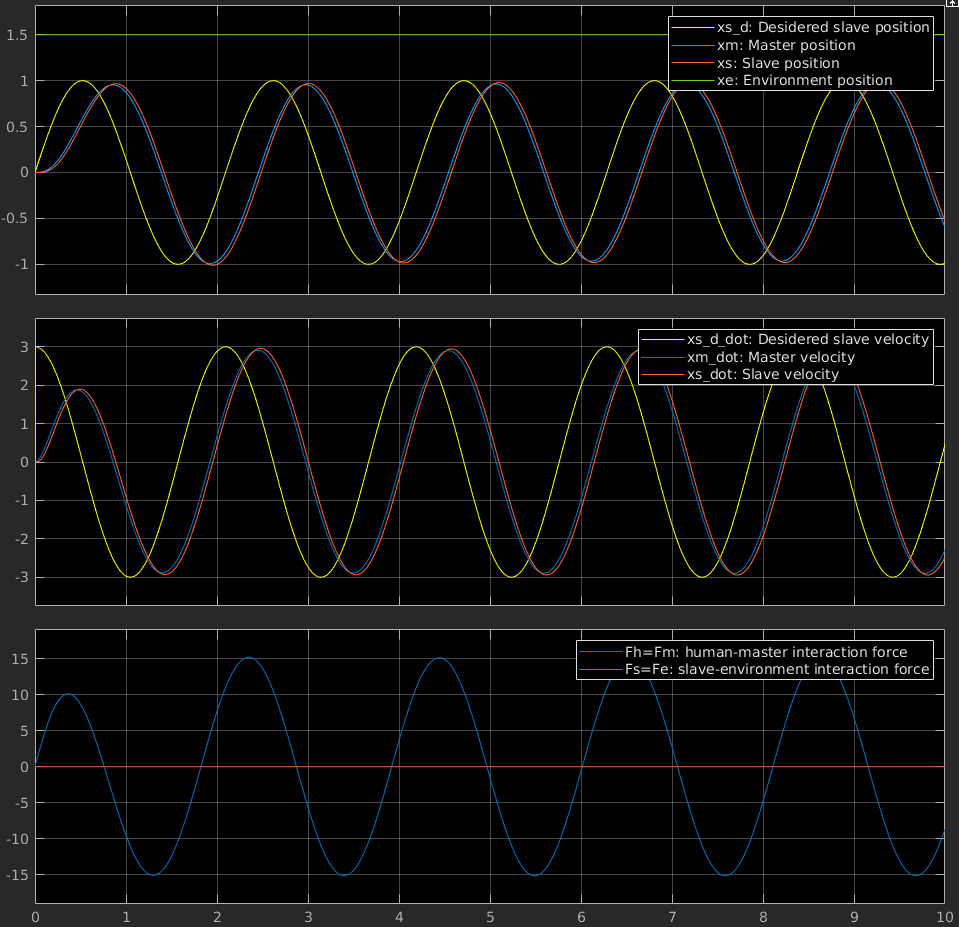
\includegraphics[keepaspectratio,width=\textwidth]{sfp_free_nok}
\caption{FP in free motion, without noise}
\label{fig:sfp_free_nok}

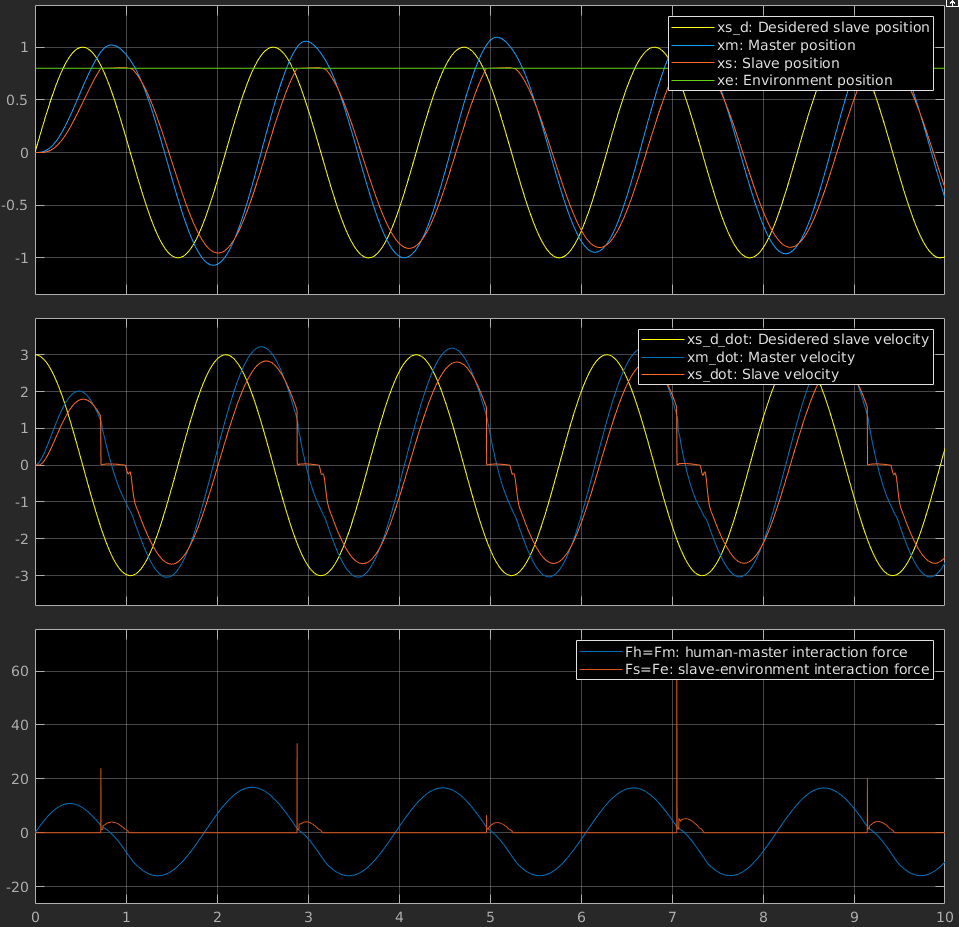
\includegraphics[keepaspectratio,width=\textwidth]{sfp_contact_nok}
\caption{FP in contact, without noise}
\label{fig:sfp_contact_nok}
\end{minipage}
\begin{minipage}{0.5\textwidth}
\centering
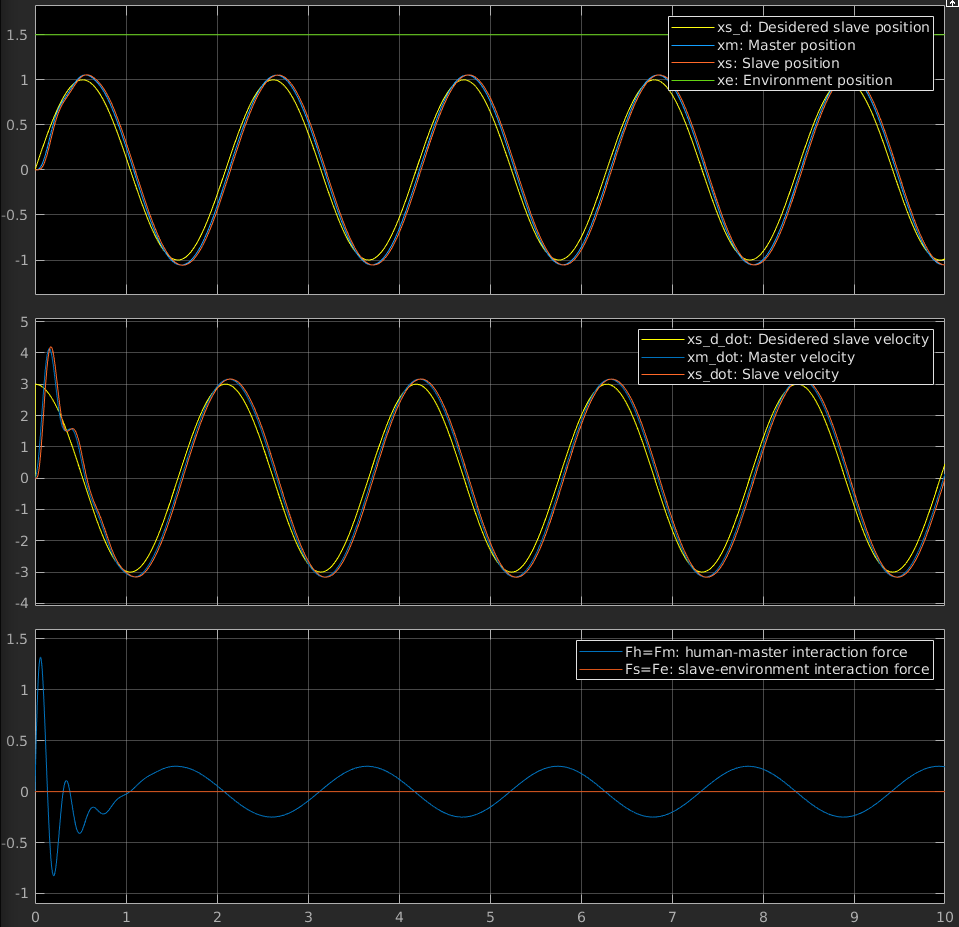
\includegraphics[keepaspectratio,width=\textwidth]{spp_free_nok}
\caption{PP in free motion, without noise}
\label{fig:spp_free_nok}

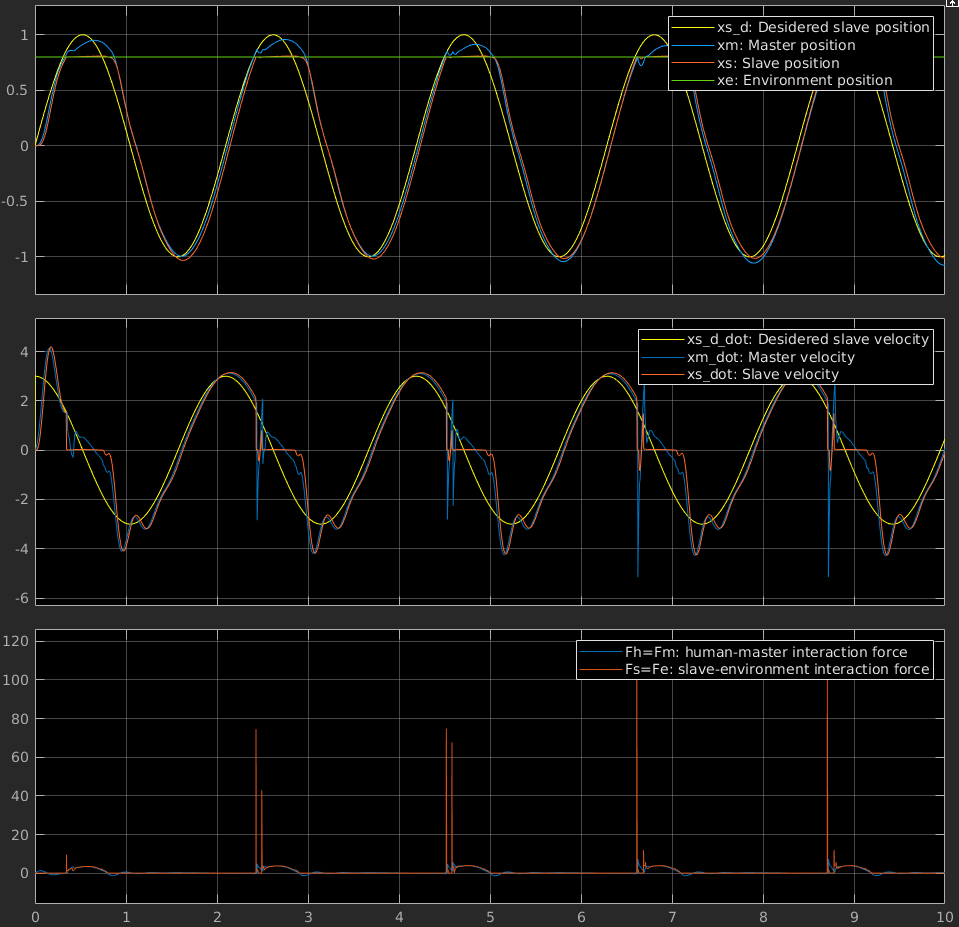
\includegraphics[keepaspectratio,width=\textwidth]{spp_contact_nok}
\caption{PP in contact, without noise}
\label{fig:spp_contact_nok}
\end{minipage}
\end{figure}

\newpage

\subsection{Create another simulink model and (a) add the measurement noise to the position/force signals, and (b) estimate velocities from positions}

\begin{figure}[H]
\begin{minipage}{0.5\textwidth}
\centering
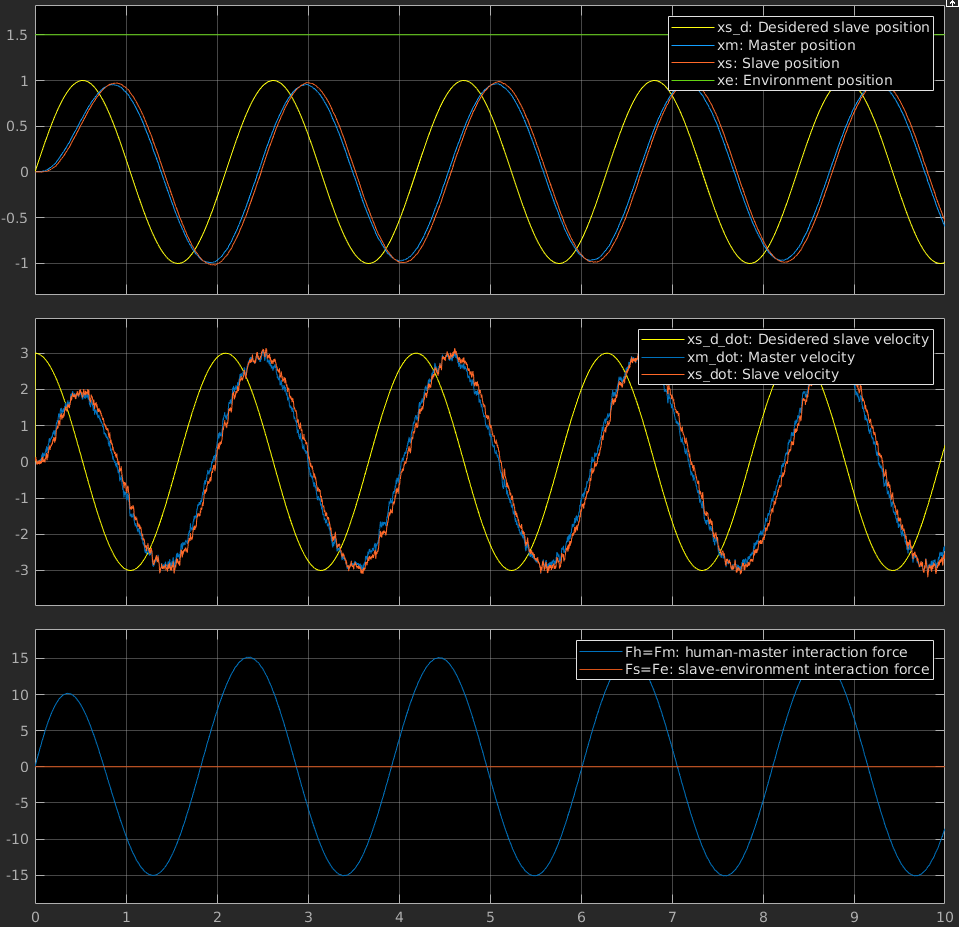
\includegraphics[keepaspectratio,width=\textwidth]{sfp_free_k}
\caption{FP in free motion, with noise}
\label{fig:sfp_free_k}

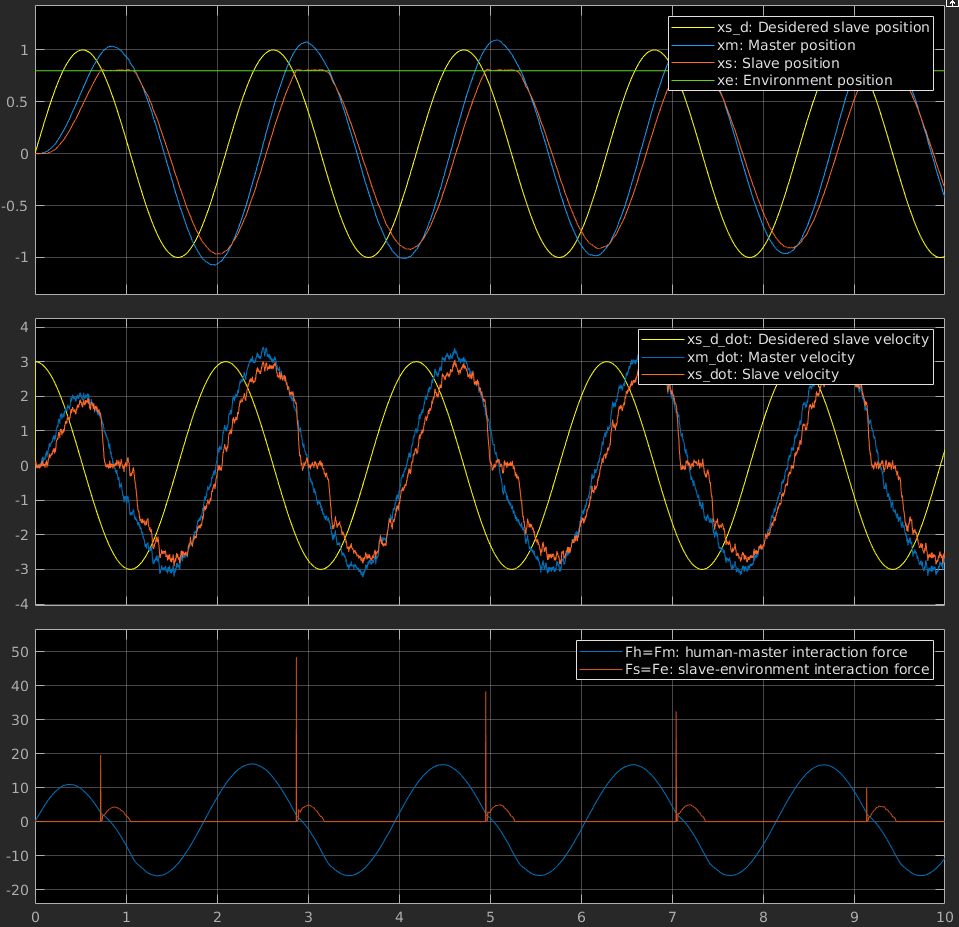
\includegraphics[keepaspectratio,width=\textwidth]{sfp_contact_k}
\caption{FP in contact, with noise}
\label{fig:sfp_contact_k}
\end{minipage}
\begin{minipage}{0.5\textwidth}
\centering
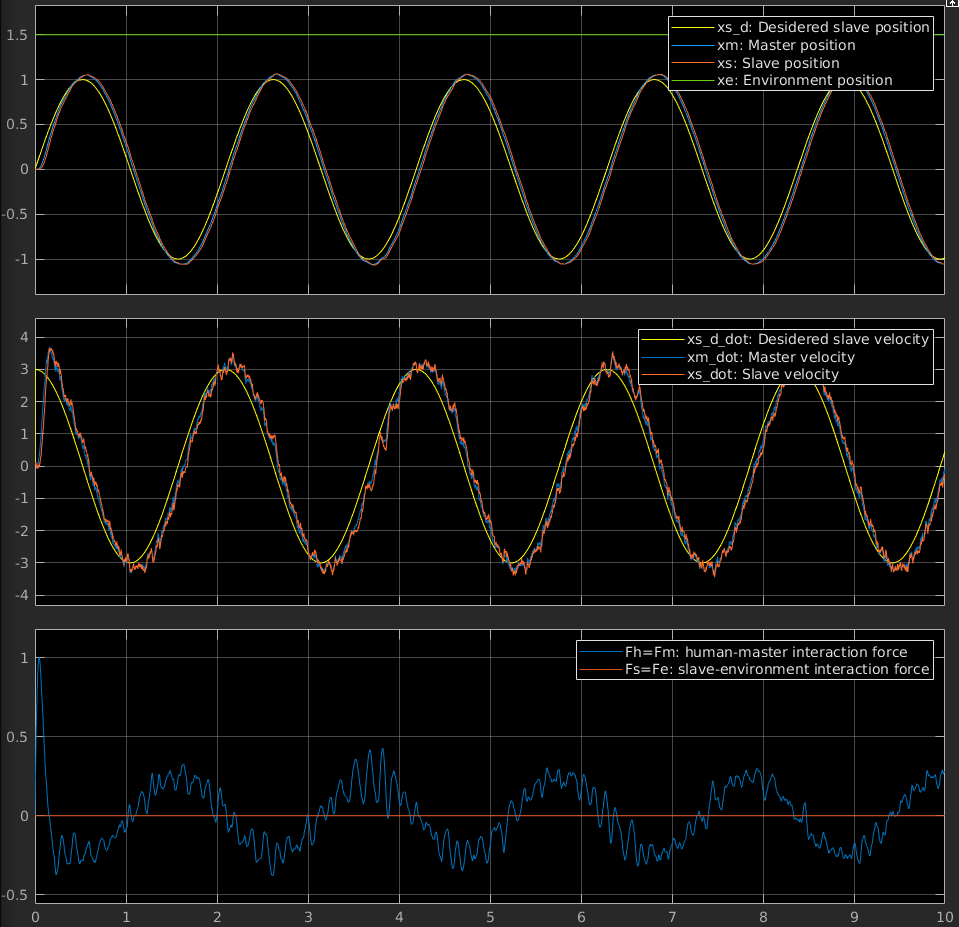
\includegraphics[keepaspectratio,width=\textwidth]{spp_free_k}
\caption{PP in free motion, with noise}
\label{fig:spp_free_k}

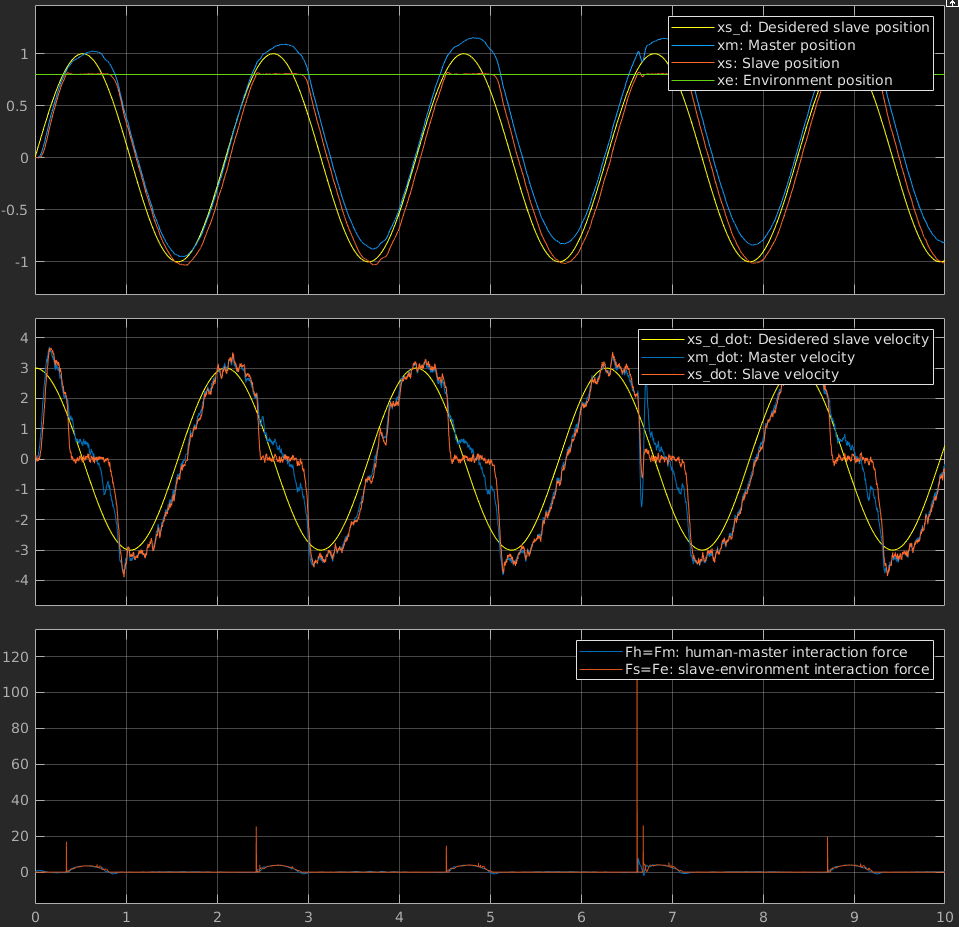
\includegraphics[keepaspectratio,width=\textwidth]{spp_contact_k}
\caption{PP in contact, with noise}
\label{fig:spp_contact_k}
\end{minipage}
\end{figure}